\documentclass[12pt,a4paper]{article}
\usepackage[utf8]{inputenc}
\usepackage{geometry}
\usepackage[english]{babel}
\usepackage[T1]{fontenc}
\usepackage{amsmath}
\usepackage{amsfonts}
\usepackage{amssymb}
%\usepackage{mathrsfs}
\usepackage{listings}
\usepackage{listingsutf8}
\usepackage{graphicx}
\usepackage{float}
\usepackage{hyperref}
\usepackage{tikz}
%\usepackage{tikz-qtree}
\usetikzlibrary{automata}
\usetikzlibrary{positioning}
\usetikzlibrary{shapes}
\usepackage{fontspec}
% disable the default 'Ligatures=TeX' option
\defaultfontfeatures{}
\setmonofont{Inconsolata}


\usepackage{minted}
\usemintedstyle{colorful}
\newmintedfile{python}{fontsize=\small,
		   linenos,
		   numbersep=8pt,
		   frame=lines,
		   framesep=3mm,
           baselinestretch=1}
\setminted{baselinestretch=1}
%\geometry{hmargin=2.0cm,vmargin=2.0cm}
\geometry{left=2.5cm, right=2.5cm, top=2.5cm, bottom=2.5cm}

\author{lemeda}
\title{Matryoshkryption - Write-up}
\date{\today}


\begin{document}
\maketitle
\vspace{4em}

\section{Description}
    \subsection{Challenge statement}
        \subsubsection{First part}
    Wow! I heard about that conf from 31C3 on file formats tweaks and the result
    is pretty impressive.\\

    Will you find what is hidden inside that matryoshka?

        \subsubsection{Second part}
    You need to solve the first part of the challenge first.

    \subsection{File provided to the challenger}
        \texttt{matryoshkryption.tgz}.

\section{Write-up}
    This section describes an example of process that could lead to solving the
    challenge.\\

    \subsection{Starting up}
    The only provided file is a \texttt{.tgz} archive.
    Once decompressed, we get a single file, named \texttt{<file\_shasum>.png}.

    \subsection{Handling the \texttt{png} file}
    An image viewer such as \texttt{feh} displays a photograph of a matryoshka.

    \begin{figure}[H]
        \begin{center}
            \fbox{\includegraphics[width=0.6\textwidth]{../../assets/matryoshka.png}}
        \end{center}
    \end{figure}

    Even though the picture itself does not seem particular in an way, some elements about the \texttt{png} file are untypical:
    \begin{itemize}
        \item[\bullet] running the \texttt{file} command on the \texttt{png} file should display informations relative to the picture (typically, something like:\\
            \texttt{<shasum>.png: PNG image data, 1400$\times$1400, 8-bit/color RGB, non-interlaced}).
            This is definitely not the case here, since the output we get is:\\
            \texttt{<shasum>.png: data}.
        \item[\bullet] the file is 5.9MB large. This is huge, all the more so
            that the picture's dimensions are 1400$\times$1400px, which is not
            particularly high. We could expect such a file to weigh a few
            hundreds of kilobytes, but not much more.
    \end{itemize}

    \vspace{1em}
    Ok, something is definitely hidden in that file (actually, we already knew that, otherwise the challenge would not have been categorized in steganography).\\

    Opening the file with a text editor shows even more weirdness: the file starts as a standard png file (see below), but the first data chunk of the file is a "\texttt{aaaa}" chunk, which is strange for at least two reasons:
    \begin{itemize}
        \item[\bullet] the first data chunk of a png file should always be the \texttt{IHDR} chunk;
        \item[\bullet] \texttt{aaaa} is not an actual chunk type.
    \end{itemize}

    \vspace{2em} {\centering%
        \fbox{
            \parbox{0.95\textwidth}{%
                \textbf{Some insights on the PNG file format}\\
                Understanding the PNG file format in detail is not necessary in order to solve this challenge, but some elements given below may help the reader get a better overview of how this step of the challenge has been built and on how to solve it.\\

                \begin{itemize}
                    \item[\bullet] To be valid, a png file must start with \texttt{$\backslash$x89$\backslash$x50$\backslash$x4e$\backslash$x47$\backslash$x0d$\backslash$x0a$\backslash$x1a$\backslash$x0a}. These bytes are the "magic number" of the PNG format and makes files in that format identifiable as such.
                    \item[\bullet] Data in png files are organized in "chunks", which are segments containing various data about the file. For instance, the \texttt{IHDR} chunk must be the first to appear in the file, and contains information such as the picture's width and height, as well as the bit depth, color type, compression method, filter method, and interlace method. This chunk is 13 bytes long. The \texttt{IDAT} chunk contains the actual data that makes the picture, and can be split into several chunks (all still called \texttt{IDAT}). The \texttt{IEND} chunk marks the end of the file.
                    \item[\bullet] Manifold types of chunks exist, some of which are required in the file for it to be valid and some of which are optional. One can add custom chunks, which will most likely be ignored by the image viewer when the file is opened. Some chunks have a fixed size, some other a variable size with a fixed limit. The other are assumed to have a variable size and must weigh less than a limit which is hardcoded in the implementations of the standard (for example, \texttt{libpng} specifies that no chunk can weigh more than 8000000 bytes).
                \end{itemize}
            }%
        }%
    }
    \vspace{2em}

    Without more information, it is a bit difficult to understand how to use
    what we have got so far. There must be something more somewhere in the
    file.\\
    A common method to hide data into an image file - referred to as the
    \textit{cover file} - consists in embedding the data to hide into the least
    significant bits of the picture - particularly if the format is lossless,
    which is the case for the \texttt{png} format.  The basic idea is that for
    each of its pixels, for one or several color components (among red, green,
    blue), the last bit of the byte representing that component of that pixel
    is replaced with a bit of the data to conceal.\\
    This method is called \texttt{LSB} (for \textbf{L}east
    \textbf{S}ignificant \textbf{B}it).\\
    A variant consists in modifying the pixels of the picture so that the data
    is embedded visually: basically, in that context, the pixels of the cover
    file are modified so that isolating the plan made of the LSBs of one or
    several color components lets appear the hidden data. For matters of clarity,
    we will refer to this technique as \textit{Visual LSB}.\\


    Let's find out whether one method or the other has been used to hide any
    data into the image.\\
    Even though we could write detection scripts to do so, a useful piece of
    software named \texttt{stegsolve} already exists to serve that purpose.
    Let's use it.\\

    Trying to open the file with \texttt{stegsolve} directly, we encounter the
    following error message: \\
    "\texttt{Failed to load file javax.imageio.IIOException: I/O error reading PNG header!}"\\
    That is probably due to the presence of the \texttt{aaaa} chunk in first position instead of the \texttt{IHDR} one. To solve that issue, a solution consists in opening the image in an image editor - such as GIMP - and to export it again to the png format.\\

    Once that done, we can finally open the picture in \texttt{stegsolve}.

%    \begin{figure}[H]
%        \begin{center}
%            \fbox{\includegraphics[width=0.5\textwidth]{./pictures/matryoshka.png}}
%        \end{center}
%    \end{figure}

    Let's start with visual LSB. Navigating between the differents plans of each component, we discover that the plan made of the LSBs of the green component holds the message "\texttt{key: <some\_key>}" and that of the blue component the message "\texttt{iv: <some\_iv>}". Both \texttt{<some\_key>} and \texttt{<some\_iv>} seem to be the hexadecimal representation of 16-byte long strings.

    % TODO: screenshot?

    That will likely prove useful, although we do seemingly not have anything to
    encrypt or decrypt yet.\\

    Let's have a look at the potential data in the "actual" LSBs of the picture
    (for instance using \texttt{Analyse > Data Extract} in \texttt{stegsolve}.
    Once again we find something interesting: more specifically, the plan made
    of the LSBs of the red component holds something that looks like a
    dictionary or a substitution alphabet.\\


    In the end, LSB methods were indeed used to conceal data in that matryoshka
    picture.  But nothing among what we have found so far provides an obvious
    hint on what to do next.\\

    Even though we don't know what to do with what we have found, it may seem
    relevant to save the different elements - for example into files called
    \texttt{png\_key}, \texttt{png\_iv} and \texttt{alphabet}.

    Since we have not got anything really more relevant to do, let's have a
    closer look at the challenge statement. It mentions a conference that was
    held at a venue called "31C3" and that addressed a topic related to file
    formats. Looking up "31C3 file formats" in a search engine, one of the
    first results links to the slides of Ange Albertini's conference "Funky
    File Formats". There are quite a lot of slides, but looking for the string
    "encryption" within them displays a single occurrence, related to a concept
    called "Angecryption". Looking for more information allows us to get a
    better understanding of it (see below).

    \vspace{2em} {\centering%
        \fbox{
            \parbox{0.95\textwidth}{%
                \textbf{Some insights on Angecryption}\\
                Angecryption was introduced by Ange Albertini in 2014. The core
                concept of it is to use the malleability one has got on the
                first plaintext block when using AES-128 CBC's decryption
                function by choosing the IV properly. More specifically, given
                a particular 16-bytes block of data considered as a ciphertext
                block, and given a chosen symmetric key, decrypting this
                ciphertext block with that symmetric key gives 16 bytes of data
                which is then xored with an IV to give the actual corresponding
                plaintext block. The IV can thus be chosen so that we get the
                value we want as plaintext block (IV $= <$output of AES$_{DEC}>
                \oplus <$desired block$>$).\\ In particular, the IV can be
                chosen so that the first block of data looks like the beginning
                of a file of another type. Of course, this comes with some
                constraints as the specifications of the target file format
                must be respected for the resulting file to be valid. More
                details can be found at
                \href{https://github.com/indrora/corkami/blob/master/src/angecryption/slides/AngeCryption.pdf}{https://github.com/indrora/corkami}
            }%
        }%
    }
    \vspace{2em}

    It thus appears very likely that what we have is some file that has been
    encrypted using angecryption with the key \texttt{<some\_key>} and IV
    \texttt{<some\_iv>} we found previously. Let's try to decrypt with the
    following script:


    \pythonfile{src/solve_angecryption.py}

    We run the following command:
    \texttt{python solve\_angecryption.py --input <png\_file>  --key png\_key --iv png\_iv --output png\_output}.\\

    Running \texttt{file png\_output}, we get the following output:\\
    \texttt{png\_output: PDF document, version .b}.

    \subsection{Handling the \texttt{pdf} file}

    Note: the \texttt{pdf} file we just obtained will be refered to as \texttt{<pdf\_file>} thereafter.\\

    Once opened in a pdf viewer, the document displays a music score written in
    C clef. The musical rules seem to be followed; however, only quarter notes
    have been used, which is a bit unusual in the sense that the resulting song
    would probably be quite boring to listen to.\\

    Anyways, listening to the resulting song is not really an option as we
    would have to generate the corresponding audio file, which would make it
    impossible for something particular to have been concealed in it.\\

    Thus, what seems to be the thing to do is to decode the music score in
    terms of notes, which semmes even more likely that we have not used the
    alphabet we found earlier. This is quite a long task, which requires focus
    and patience, but is not too complex to achieve.\\

    Once the music score decoded into a more textual form, we can put the
    alphabet in a way that makes it suitable for it to be handled by a script -
    for instance in the Python language. Afterwards, the only thing left to do
    is to use our substitution alphabet on our encoded message to get to
    something more understandable.\\

    We thus obtain a message which gives us a new key/iv pair - which we can
    save in files named \texttt{pdf\_key} and \texttt{pdf\_iv}, as well as a
    flag, and a piece of advice stating that the pdf document might still be of
    use.\\

    \textbf{The flag we got validates the first part of the challenge}.\\

    Having a closer look at the document, we notice that at the very end of it,
    some kind of copyright line is written. However, the second part of it is
    not intelligible, and its form suggests it is a base-64-encoded message.
    Once decoded - for example with \texttt{echo -en <b64\_encoded\_message> |
    base64 --decode}, we get a passphrase, that we can save as
    \texttt{passphrase}.\\

    Since there is nothing obvious we can do with that passphrase, let's use
    the key/iv air we have found to get to the next step. The PDF document is
    likely another angecryption-encrypted file, so we use the same script as
    before with our new key/iv pair to try and find what is conceal in it:\\
    \texttt{python solve\_angecryption.py --input pdf\_file --key pdf\_key --iv
    pdf\_iv --output pdf\_output}.\\

    Running \texttt{file pdf\_output}, we get: \texttt{pdf\_output: MPEG ADTS,
    layer III, v1, 128 kbps, 44.1 kHz, Monaural}.\\
    The next file thus appears to be an audio file. After a quick search, we
    understand that its format is more or less equivalent to the \texttt{mp3} format.


    \subsection{Handling the \texttt{mp3} file}
    Note: in that section and thereafter, the \texttt{mp3} file we just
    obtained will be refered to as \texttt{<mp3\_file>}.\\

    Listening to the \texttt{mp3} let us hear a morse-encoded message. At some
    point, we can also notice some additional noise.\\
    Opening the file in Audacity makes it easier to decode the morse message
    since it provides us a way to visualize the file and thus to decode each
    character more conveniently. However, doing this requires the
    not-so-convenient step of understanding that our file is in the
    \texttt{mp3} format (or something close) and renaming the file to something
    that holds the "\texttt{.mp3}" extension.\\
    Decoding the morse message gives us a new key - we save it
    in a \texttt{mp3\_key} file.\\

    Having a look at the "noisy" part of the file does not directly reveal
    anything interesting. However, by switching to the \texttt{Spectrogram}
    view, we notice that something seems to be written there. After making the
    adequate adujstments to the view, we get a new IV, which we save to
    \texttt{mp3\_iv}.\\

    Once again, let's try to de-angecrypt our file with the new key/IV pair:\\
    \texttt{python solve\_angecryption.py --input mp3\_file --key mp3\_key --iv
    mp3\_iv --output mp3\_output}.


    Running \texttt{file mp3\_output}, we get:\\
    \texttt{mp3\_output: ISO Media, MP4 Base Media v1 [IS0 14496-12:2003]}.\\
    The next file thus appears to be an \texttt{mp4} file.


    \subsection{Handling the \texttt{mp4} file}
    Note: in that section and thereafter, the \texttt{mp4} file we just
    obtained will be refered to as \texttt{<mp4\_file>}.\\

    Watching the video informs us about something that occurred at the end of January, but does not provide us really useful information. Using tools such as \texttt{binwalk} does not help more, and looking at the bytes of the file by ourselves shows nothing useful either.\\

    Since we can seemingly not use the file on its own, let's think for one
    second about elements that could help. We have used every auxiliary element
    we have found in the previous steps, except the string that looked like a
    potential passphrase that we got from the pdf document. That passphrase
    being the only unused element, it is very likely to be used in that step in
    some way. Nevertheless, we still do not know how to use it.\\

    Let's have a closer look at it: we can note that there is something weird
    with the type case of it: it is mostly written in CamelCase but some
    characters are in uppercase even though they are not at the beginning of a
    word and some are in lowercase whereas they are at the beginning of a word.
    We can then notice that the part of the passphrase that has been altered
    seems to highlight the message "TrueCrypt". Searching for "TrueCrypt mp4"
    in a search engine displays that a TrueCrypt volume can easily be hidden in
    an mp4 file.\\

    Trying to mount the mp4 file as a TrueCrypt volume proves vain, as the
    video is not recognized as a TrueCrypt volume. However, looking for more
    information about TrueCrypt makes us aware that TrueCrypt has been
    deprecated for a while, and that a common alternative to it is VeraCrypt.\\

    Trying to mount the mp4 file as a VeraCrypt volume with the following
    command proves successful:\\
    \texttt{veracrypt -p passphrase --mount mp4\_file <mountpoint>}.\\
    Inside the volume, we find a single file named \texttt{flag}.\\

    \textbf{The content of the \texttt{flag} file validates the second part of the challenge}.


\end{document}
